% !TEX program = pdflatex
\documentclass[10pt,a4paper,twocolumn]{article}

% ---------- Look & feel ----------
\usepackage[left=1.6cm,right=1.6cm,top=1.6cm,bottom=1.9cm]{geometry}
\setlength{\columnsep}{0.64cm}
\setlength{\parindent}{0pt}

\usepackage{newpxtext,newpxmath}  % sleek serif text/math
\usepackage[scaled=0.92]{DejaVuSansMono}
\usepackage[T1]{fontenc}
\usepackage[utf8]{inputenc}
\usepackage{microtype}
\usepackage{xcolor}
\usepackage{hyperref}
\hypersetup{colorlinks=true,linkcolor=black,citecolor=black,urlcolor=black}
\usepackage[capitalise,noabbrev]{cleveref}
\usepackage{graphicx}
\usepackage{subcaption}
\usepackage{booktabs}
\usepackage{enumitem}
\usepackage{amsmath,amssymb}
\usepackage{csquotes}
\usepackage{titlesec}
\usepackage{titling}
\usepackage{ragged2e}
\usepackage[labelfont=bf,font=small]{caption}

% tighter headings
\titlespacing\section{0pt}{8pt plus 2pt minus 2pt}{6pt plus 2pt minus 2pt}
\titlespacing\subsection{0pt}{6pt plus 2pt minus 2pt}{4pt plus 1pt minus 1pt}
\titleformat{\section}{\large\bfseries}{\thesection}{0.6em}{}
\titleformat{\subsection}{\normalsize\bfseries}{\thesubsection}{0.6em}{}

% subtle link underline for urls in references (optional)
\usepackage[normalem]{ulem}
\renewcommand{\ULdepth}{1.8pt}

% small helper to draw figure placeholders
\newcommand{\figph}[2][2.1in]{%
  \fbox{\parbox[c][#1][c]{0.96\linewidth}{\centering \vspace{0.5em}\textit{#2}\vspace{0.5em}}}%
}

% inline TODOs (remove before submission)
\newcommand{\todo}[1]{\textcolor{magenta}{[\textbf{TODO}: #1]}}

% ---------- Title ----------
\setlength{\droptitle}{-8pt}
\pretitle{
  \begin{center}
  \rule{\linewidth}{0.75pt}
  \par\vspace{12pt}
  \fontsize{14}{16}\selectfont\bfseries
}
\posttitle{\par\vspace{4pt}\rule{\linewidth}{0.75pt}\end{center}}
\preauthor{\par\vspace{7pt}\begin{center}\normalsize}
\postauthor{\end{center}}
\predate{}\postdate{}

\title{Temporal Predictors of Outcome in Reasoning Language Models}
\author{
  \textbf{Joey David} \\[1pt]
  Independent Researcher \\[1pt]
  joeydhp@protonmail.com
}
\date{}

\begin{document}
\maketitle
\vspace{10mm}

% ---------- Abstract ----------
\renewenvironment{abstract}{
  \begin{center}
  \begin{minipage}{0.9\columnwidth}
  \centering{\large\bfseries\abstractname}
  \par\vspace{14pt}
  \justifying
  \ignorespaces
}{
  \end{minipage}
  \end{center}
}

\begin{abstract}
The chain-of-thought (CoT) paradigm uses the elicitation of step-by-step rationales as a proxy for reasoning, gradually refining the model’s latent representation of a solution. However, it remains unclear just how early a Large Language Model (LLM) internally commits to an eventual outcome. We probe this by training linear classifiers on hidden states after the first $t$ reasoning tokens, showing that eventual correctness is highly predictable after only a few tokens, even when longer outputs are needed to reach a definite answer. We show that, for harder questions, a drop in predictive accuracy highlights a selection artifact: hard items are disproportionately represented in long CoTs. Overall, our results imply that for reasoning models, internal self-assessment of success tends to emerge after only a few tokens, with implications for interpretability and for inference-time control.
\end{abstract}

\par\vspace{10pt}

% ---------- 1. Introduction ----------
\section{Introduction}
\label{sec:intro}

Late 2024 and early 2025 saw the first large-scale implementations of CoT finetuning and prompting, notably in OpenAI's \textit{o1} \cite{openai2024openaio1card} and Deepseek's \textit{R1}\cite{deepseekai2025deepseekr1incentivizingreasoningcapability} models. This led to LLMs achieving unheard-of performance in cognitively demanding tasks, especially in mathematical problem-solving and commonsense reasoning. The mechanism behind these improvements consists in pushing the model to generate a step-by-step path to a solution, openly formulating calculations or deductions, possibly reflecting on possible mistakes that could be made along the way before settling on a final answer. CoT generations are not mechanistically different from \textit{regular} token generation; they are simply specialized to problem-solving. Thus, deciding whether a model's latent representation has already converged onto a definite answer, or whether all of the CoT remains necessary to reach it, is an important but non-trivial problem. A model able to assess when it is honing in on the right solution may enable early error detection, better calibration, or dynamic halting of reasoning to save computation \cite{mao2025earlystoppingchainofthoughtslarge}.

% ---------- Fig 1 (answer length vs accuracy) ----------
\begin{figure}[t]
  \vspace{1.5cm}
  \centering
  \makebox[\columnwidth][c]{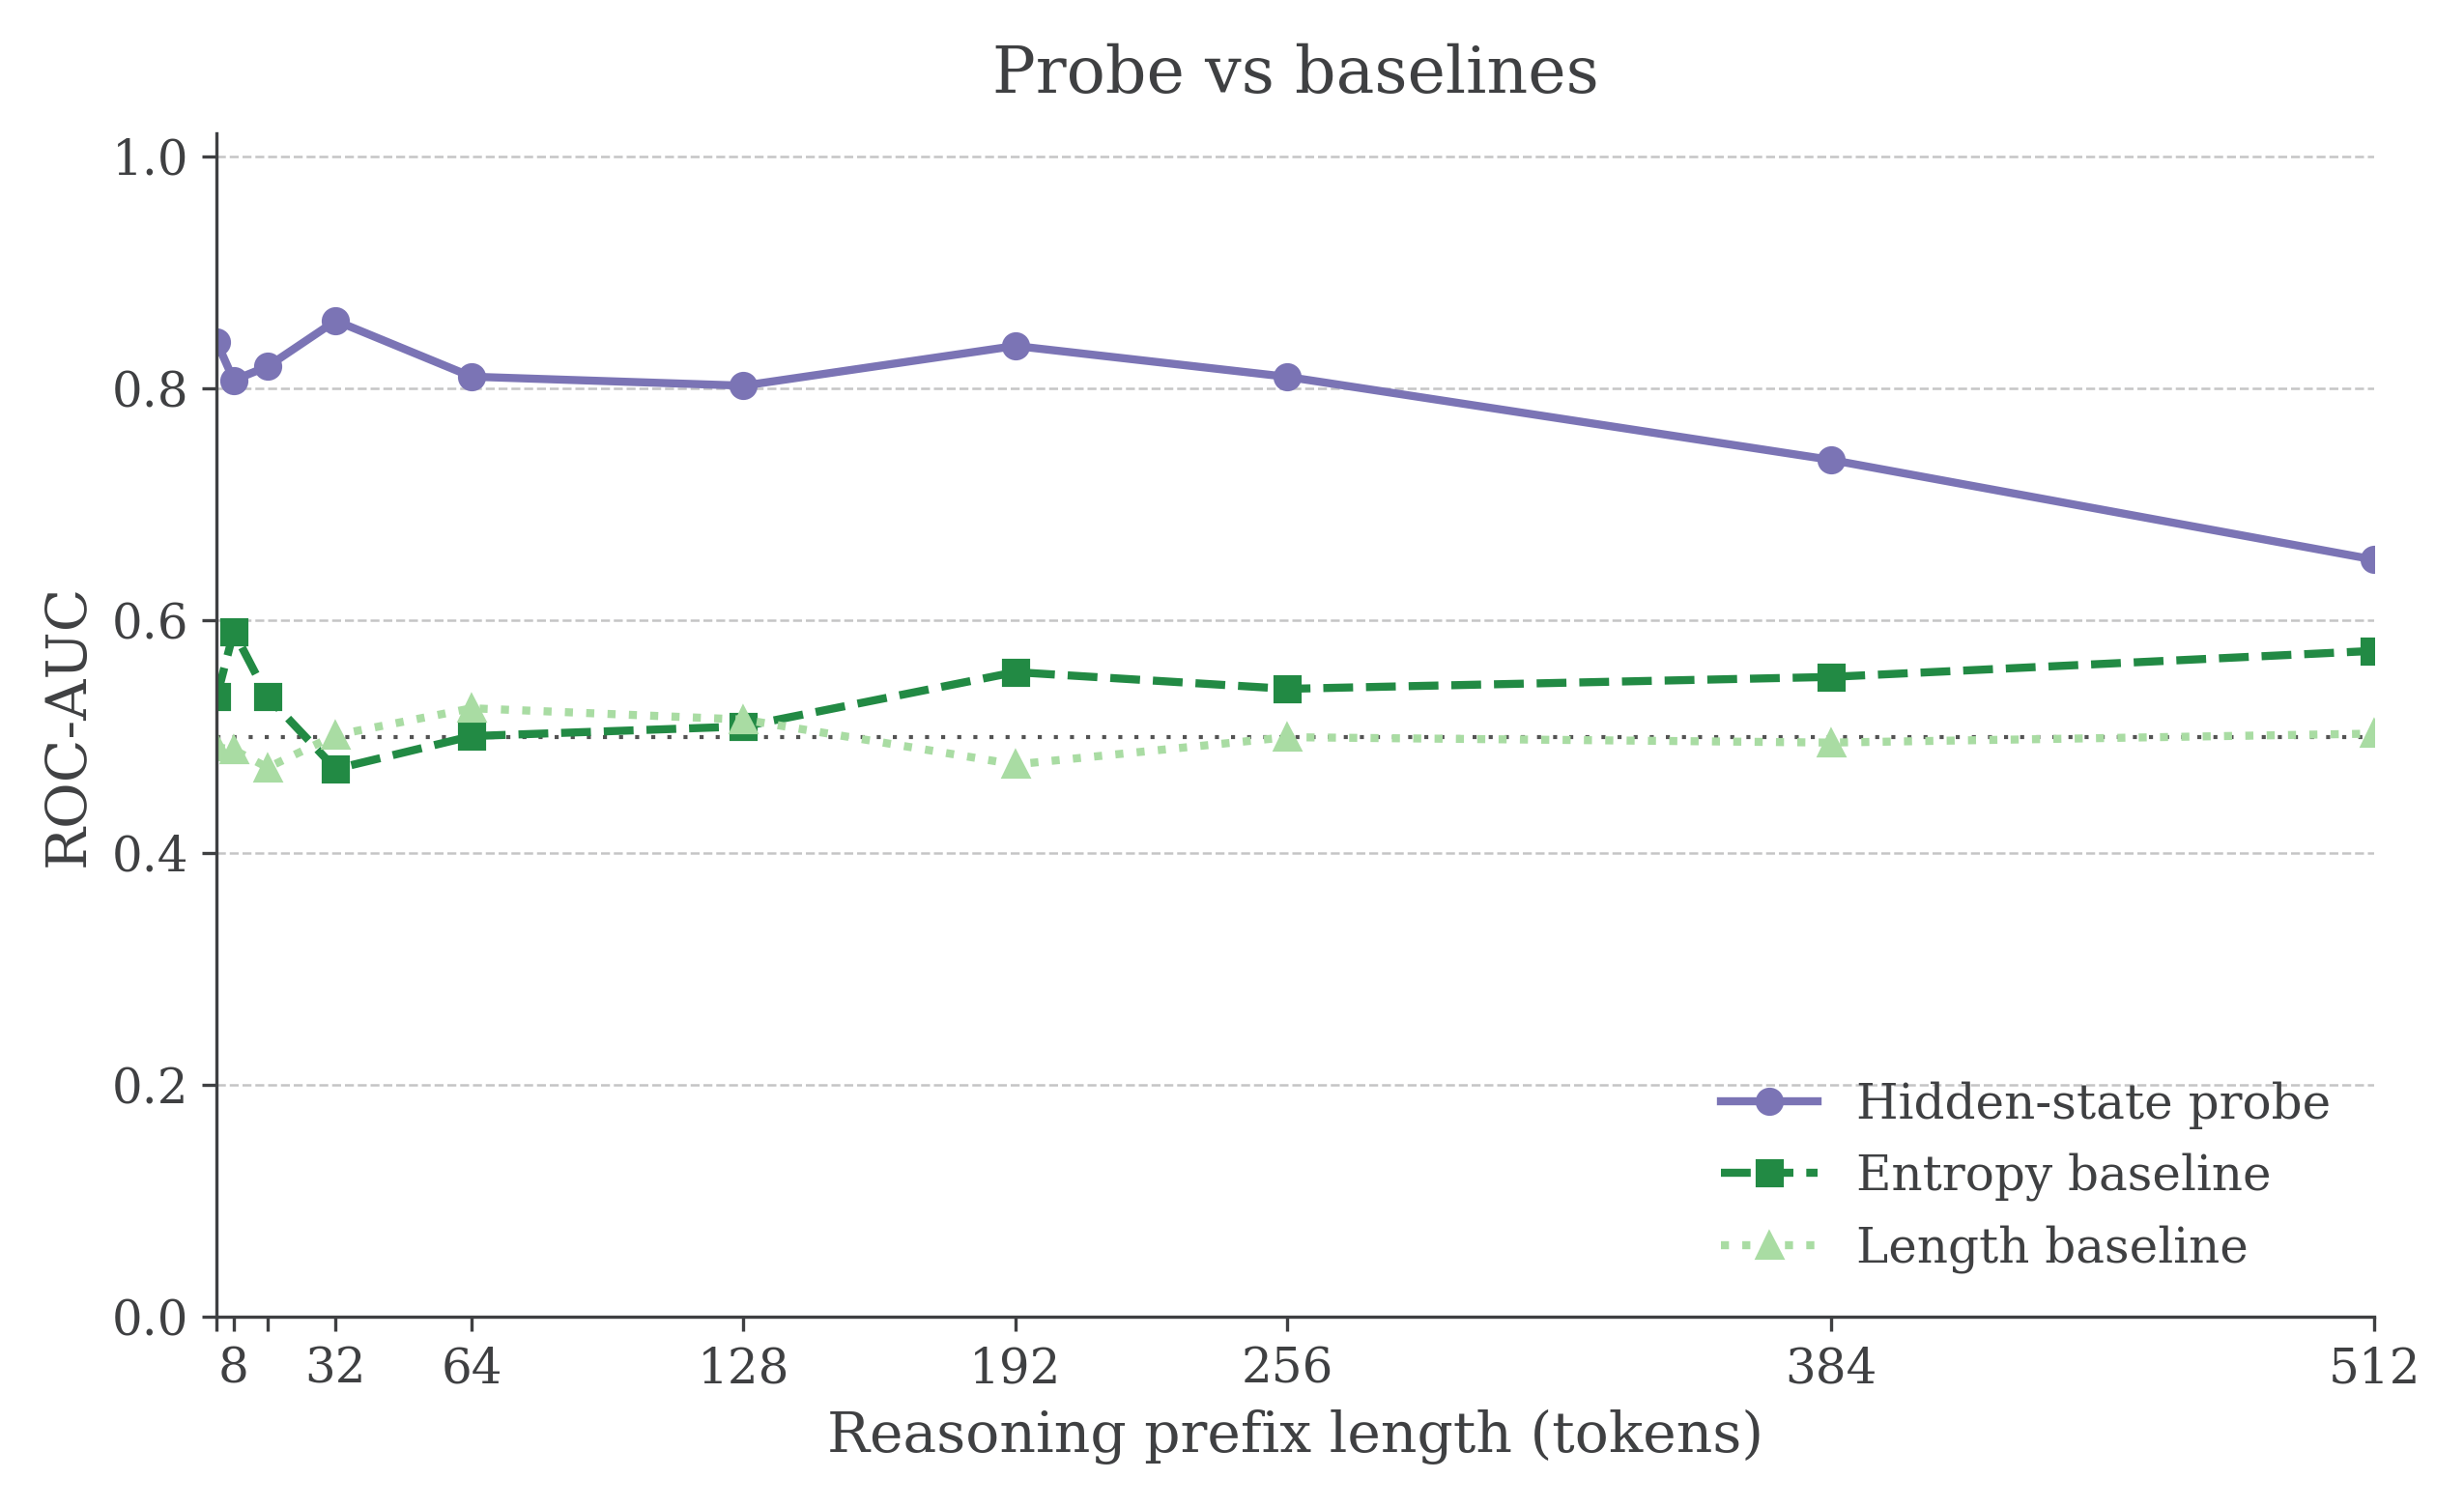
\includegraphics[width=1.05\columnwidth]{Qwen3-8B_baselines.png}}
  \caption{Probe performance vs. entropy and length baselines, depending on CoT length.}
  \label{fig:raw-cf}
\end{figure}


In this work, we attempt to answer whether such an insight can be achieved, by probing the hidden states of an LLM at several points during the generation of its chain-of-thought. Our experiments reveal a surprising result - a detectable correctness signal generally emerges very early into the reasoning process, even for longer CoT outputs. To ensure robust evaluation, we compare probe performance on the same set of problems across different prefix lengths $t$. Our analysis confirms that the model’s internal state truly encodes, to a significant extent, whether the answer will be correct well before outputting it.

Finally, we highlight how our approach differs from existing methods. Prior works on confidence estimation largely rely on post-hoc signals (the final answer logits or multiple sampled solutions) and added mechanisms at inference time. In contrast, we directly probe the model’s own hidden trajectory during reasoning, without requiring any extra decoding passes or fine-tuning of the model. Our results show that a simple linear probe is enough to tap into the model’s self-monitoring capabilities. By focusing on challenging long-form math problems, we uncover an early internal self-assessment that was previously elusive (earlier question-only probes struggled on math). In summary, our contributions include:

\begin{itemize}[leftmargin=1em]
  \item \textbf{Probing during generation:} We develop a methodology to predict answer correctness from an LLM’s hidden state throughout the generation of its chain-of-thought, rather than only after the final answer. This allows us to assess the model’s internal confidence in real time as it reasons.
  \item \textbf{Early correctness signal:} We identify a reliable latent signal of correctness after only a few tokens of reasoning (around 4 tokens in our experiments), indicating that the model’s internal computation encodes outcome likelihood far earlier than its verbalized solution.
  \item \textbf{Difficulty-dependent evaluation:} We demonstrate that harder problems not only lead to lengthier CoT generations, but also to sparser signals of confidence.
\end{itemize}


% ---------- 2. Related Work ----------
\section{Related Work}
\label{sec:related}

\subsection{Probing hidden activations for correctness and factuality.}

A growing line of work shows that LLM hidden states encode latent information about truthfulness and correctness that may not surface in its token-space output.\cite{cencerrado2025probe} extract the residual activation right after the question is processed by the model (i.e., before any answer token is produced) and train a linear probe to predict whether the model’s eventual answer will be correct. While able to reach above-chance success prediction on trivia-style QA, subsequent results of this work suggest that mathematical reasoning makes it harder to linearly decode internal confidence. Our work expands on this, and targets this gap by (i) focusing on math CoT and (ii) probing hidden states \emph{during} the reasoning trajectory, not only in the pre-answer state.

Similarly, \cite{gekhman2024insideout} introduce the \textit{Inside-Out} framework to quantify factual knowledge stored in hidden representations. They show that models frequently encode more correct facts internally than they actually express, with hidden representations yielding markedly higher recall than the generated text. Remarkably, they show that a model can internally embed a fact (with the correct answer being ranked highest in latent space) yet systematically fail to output it. These results strengthen the view that latent activations contain rich information signals, not fully exploited by standard decoding. We build on this observation in the context of CoT reasoning.

\subsection{Early stopping in CoT reasoning.}

Long CoT traces are expensive, and several methods try to stop decoding once the answer is effectively determined. ES-CoT \cite{mao2025escot} asks the model for its current answer at several points during the procedure; using the length of the resulting \textit{step-answer} compared to other step-answers as a criterion for convergence. While this approach yields substantial token savings with minimal accuracy loss, it relies entirely on output-space heuristics and does not exploit the model's internal signals. This behavior could lag behind the model's internal confidence, and the model might already carry a signal unique to the answer before it begins to repeat it in output. HALT-CoT \cite{laaouach2025haltcot} instead monitors the entropy of the next-answer distribution and stops when entropy falls below a threshold, cutting 15–30\% of tokens on GSM8K while keeping accuracy within about 0.4 points of full CoT. By contrast, our probe uses \emph{internal} signals: it aims to predict correctness from the hidden state \emph{before} the answer has converged. This potentially enables even earlier interventions—e.g., switching to self-reflection or to an alternative decoding strategy as soon as the internal probe flags low confidence; making our method complementary to ES-CoT and HALT-CoT. 

\subsection{Latent Reasoning and CoT}

Our work builds on chain-of-thought prompting \cite{wei2022chain}, which showed that providing structured intermediate steps allows LLMs to solve arithmetic and logical problems with much greater consistency than naïve prompting. Prior CoT research has noted that longer reasoning is not always better—models can “overthink” easy questions and introduce errors in late steps \cite{kojima2022large, zhou2023leastto}. This observation motivates internal progress monitoring: if the model’s activations early in the trajectory already suggest high eventual correctness, we could truncate or adapt the reasoning on the fly. To the best of our knowledge, our results are among the first to show that in complex multi-step math settings, partial CoT hidden states are greatly decodable for eventual correctness.

% ---------- 3. Method ----------
\section{Method}
\label{sec:method}
\subsection{Difficulty-balanced data}

% ---------- Fig 1 (probe) ----------
\begin{center}
\begin{minipage}{1.02\columnwidth}
  \centering
  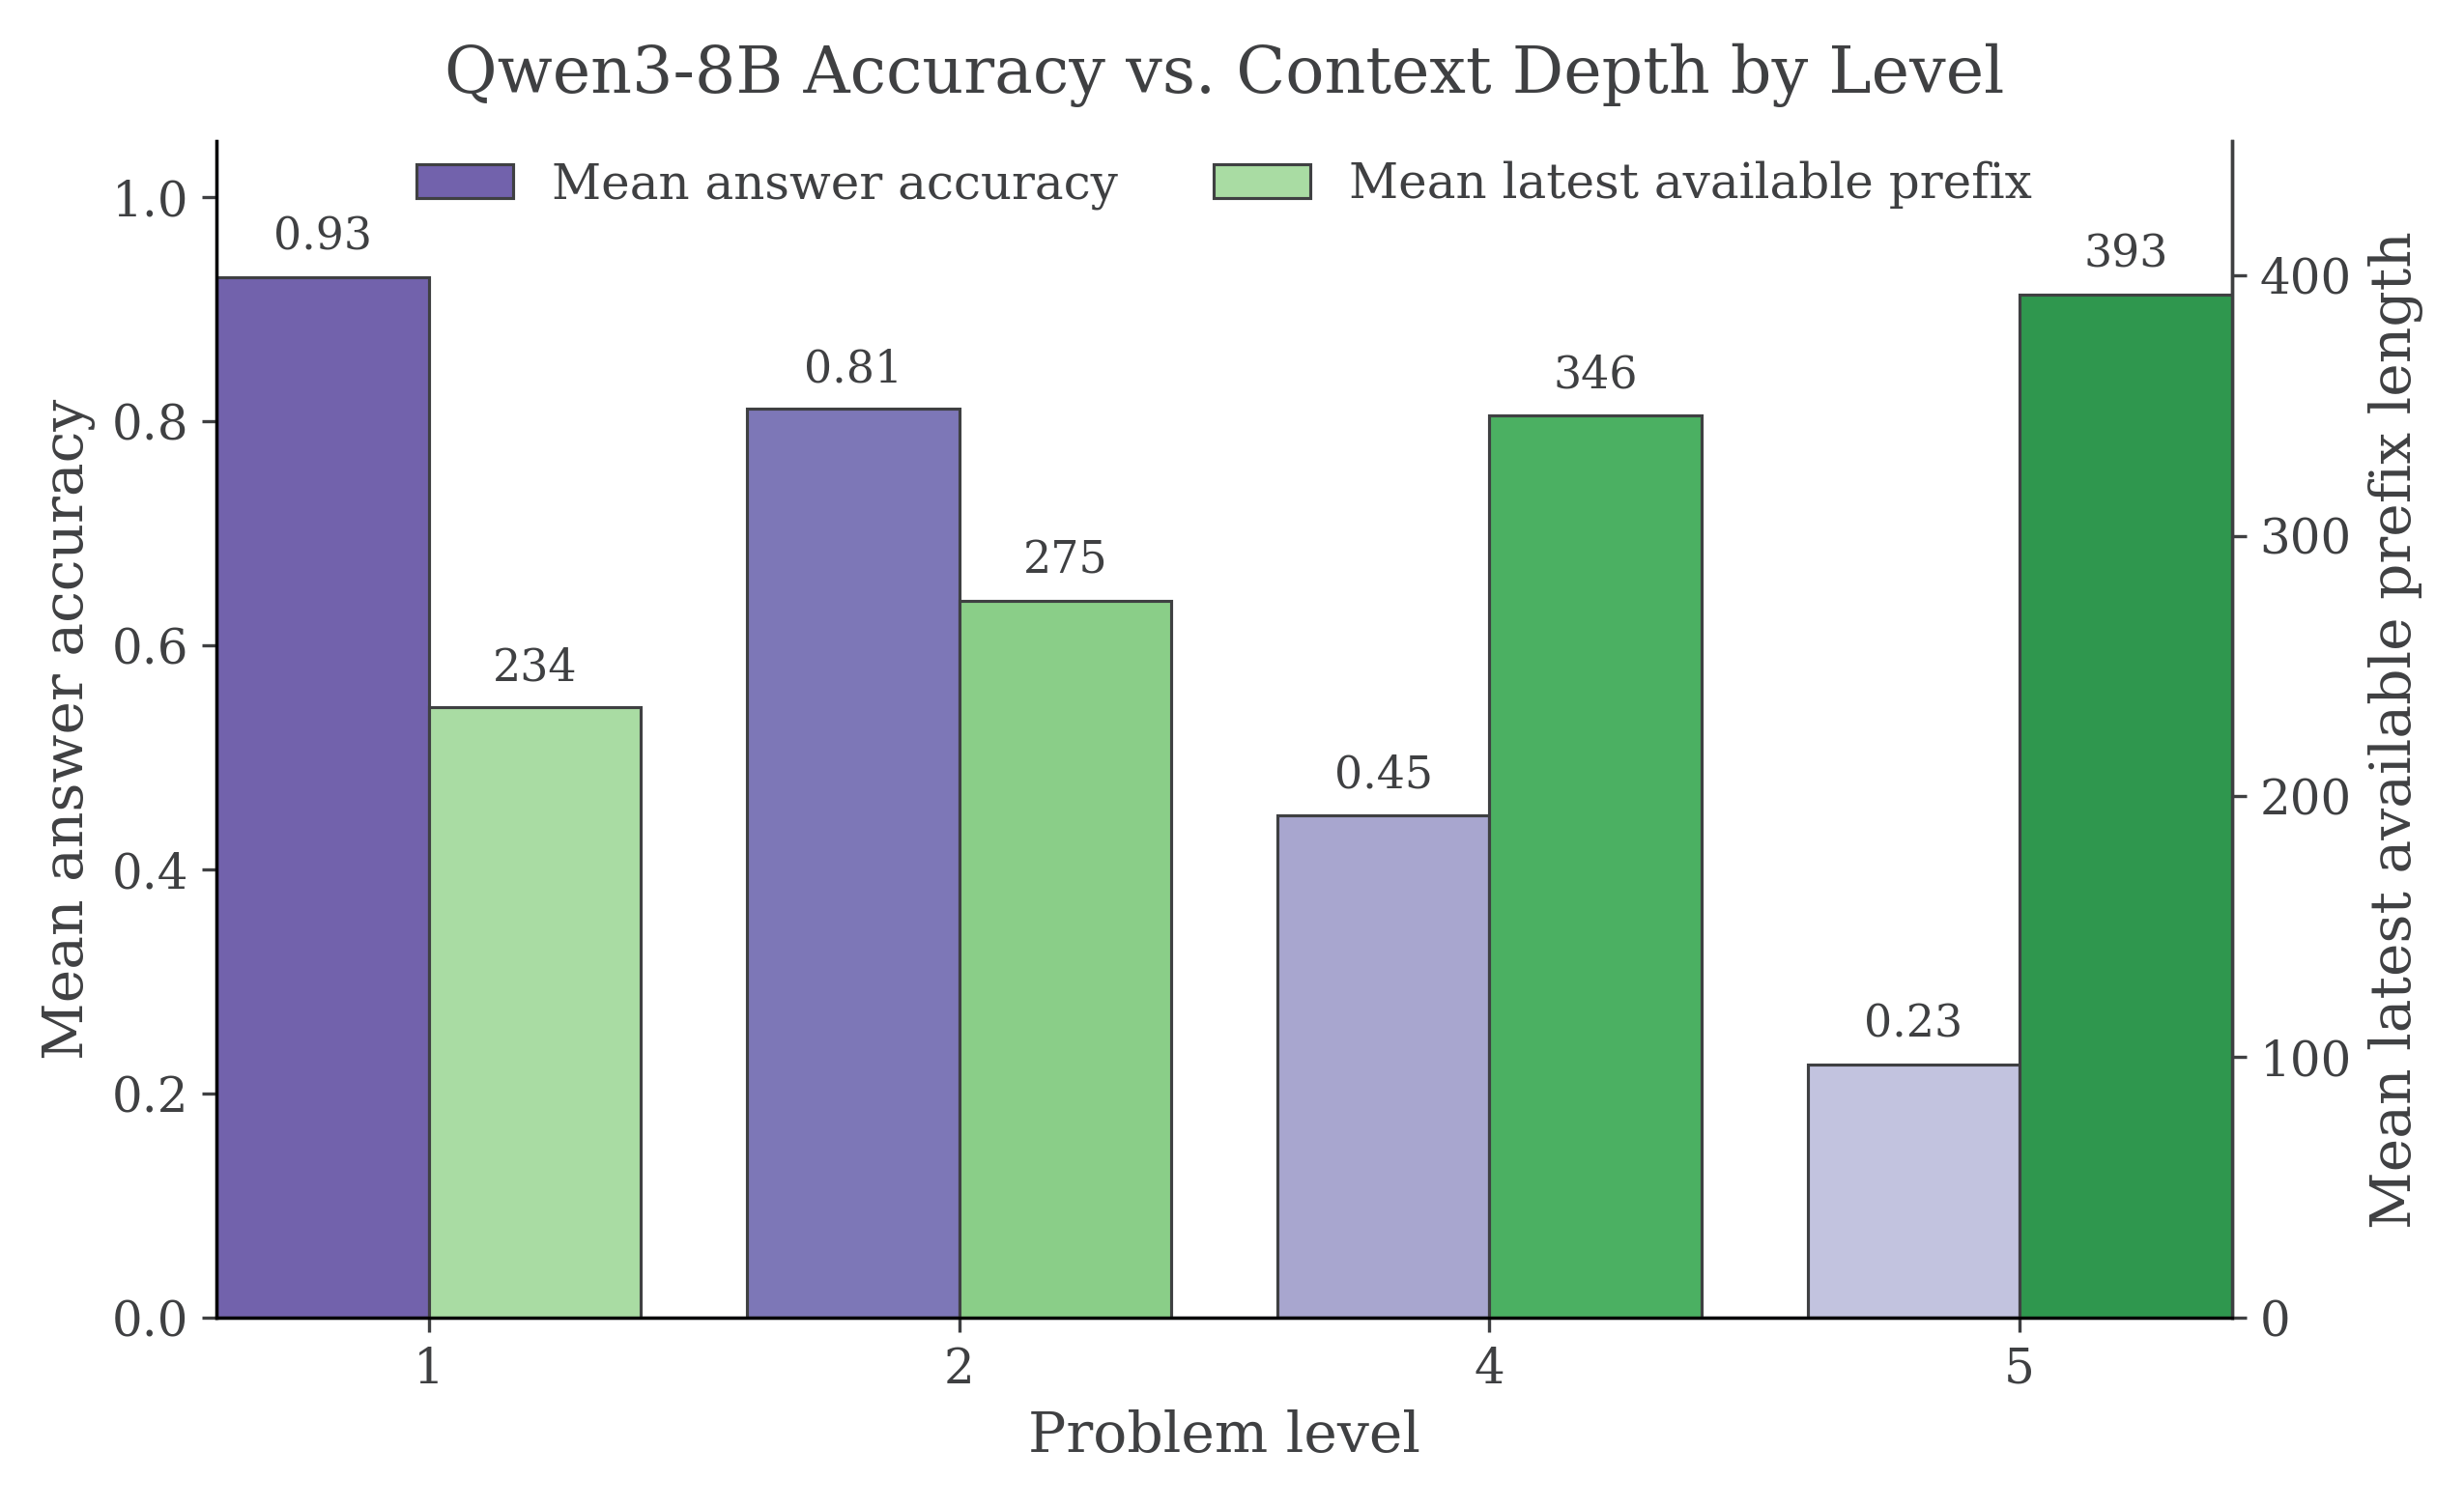
\includegraphics[width=\linewidth]{qwen_level_metrics.png}
  \captionof{figure}{Mean accuracy and CoT length per difficulty level.}
  \label{fig:raw-cf}
\end{minipage}
\end{center}


We study Hendrycks MATH \cite{hendrycksmath2021} using the helpers in \texttt{data.py}.  All seven subjects are streamed through \texttt{load\_math\_split}, which filters to numerically normalisable gold answers via lightweight LaTeX stripping and fraction simplification.  We follow the code path in \texttt{sample\_balanced\_by\_difficulty}: levels~1--2 populate the \emph{easy} bucket, and levels~4--5 the \emph{hard} bucket.  From the resulting pool we draw 750 problems per bucket, yielding 1{,}500 examples. Qwen3-8B solves easy instances 85.1\% of the time, while hard ones drop to 32.1\%, giving a wide accuracy dynamic for probing latent confidence.

\subsection{Prompting and chain-of-thought harvesting}
Question prompts are produced by \texttt{build\_prompt}.  For Qwen3 series models, we enable the structured reasoning mode: the system message instructs the model to think inside \verb|<think>...</think>| before emitting a boxed numeric answer.  Generation is handled by \texttt{generate\_cot}, which performs greedy decoding (\texttt{temperature}=0, \texttt{max\_new\_tokens}=512).  When the raw completion either omits a boxed answer or leaves the thinking span unclosed, we append a deterministic suffix (\texttt{FORCED\_SUFFIX\_SUFFIX}) and continue for up to 32 extra tokens.

\subsection{Prefix hidden-state extraction}
For every generated solution, we parse activations at fixed prefix lengths $t \in \{4,8,16,32,64,128,192,256,384,512\}$ using \texttt{get\_prefix\_hidden\_states}.  The function replays the prompt plus the first $t$ generated tokens, captures the final decoder layer, and averages the last four reasoning tokens to obtain a pooled hidden vector $h_t$.  We also log the next-token entropy and log-probability at each checkpoint.  Short prefixes are available for all items (1{,}500 slices at $t{=}4$ and $8$), and coverage gradually shrinks as chains terminate (566 examples remain at $t{=}512$).

\subsection{Labeling and leakage controls}
Correctness labels follow \texttt{compute\_correct\_label}.  Gold answers are normalized with \texttt{normalize\_num\_str}. A prefix is discarded if the gold-normalized answer string already appears in its decoded text, or if the model has already closed the \verb|</think>| block.  For the present runs, no prefix under $t{=}256$ triggers this filter, confirming that early probe accuracy is not driven by trivial answer leakage.

\subsection{Linear probe and evaluation protocol}
Hidden-state features are aggregated per checkpoint and fed to \texttt{run\_all\_probes}.  Each probe performs PCA down to at most 128 components (or fewer when the train split is smaller), then fits an $\ell_2$-regularised logistic regression with \texttt{liblinear}.  We stratify an 80/20 split and balance class weights to offset label skew.  Evaluation reports accuracy and ROC-AUC alongside the class prior in the training fold.


% ---------- 4. Experiments ----------
\section{Experiments}
\label{sec:experiments}

\subsection{Experimental setup}
All reported numbers come from the balanced MATH split described in \cref{sec:method}.  We run the end-to-end pipeline with Qwen3-8B as the reasoning model, greedy decoding, and the checkpoint grid $t \in \{4,\ldots,512\}$.  Probe features are cached in-memory during the sweep; metrics, baselines, and diagnostics are persisted under \texttt{results/}, and plots under \texttt{figs/}. Because long reasoning chains are rarer, the effective sample size drops from 1{,}500 prefixes at $t{=}4$ to 566 at $t{=}512$ (see \cref{tab:stats}).

\subsection{Prefix-wise probe accuracy}
The probe is already highly predictive after four reasoning tokens: \cref{fig:prefix} shows an ROC-AUC of 0.84 and an accuracy of 0.76 at $t{=}4$.  Accuracy dips slightly at $t{=}8$ before climbing to its peak near $t{=}32$ (0.79 accuracy, 0.86 ROC-AUC).  Longer traces yield noisier statistics because fewer examples survive---beyond $t{=}256$ the label distribution becomes skewed toward incorrect answers as only genuinely hard questions remain.  Applying the carry-forward diagnostic keeps the early AUC plateau at 0.858, and the fixed-prefix subset (requiring availability through $t{=}256$) maintains AUC~$>0.82$, indicating that the strong early signal is not an artifact of shorter solutions exiting the pool.  The carry-forward trend is summarised in \cref{fig:carryforward}.


\subsection{Difficulty and CoT-length effects}
Difficulty stratification confirms that the probe mirrors how quickly the base model commits to an answer.  At $t{=}4$ the AUC is 0.77 on easy items and 0.72 on hard items; by $t{=}32$ the gap widens (0.84 vs.\ 0.76).  Hard problems therefore require longer prefixes before their internal state separates correct from incorrect trajectories.  When we additionally condition on long chains (\textit{fixed $\leq\!256$}), the early AUC stays above 0.84, revealing that the information is already present even when we force every example to continue reasoning.  The bar chart in \cref{fig:difficulty} visualises these trends.

\subsection{Comparison with output-space baselines}
Next-token entropy and prefix length provide weak signals relative to the hidden-state probe.  Even when combined (\textit{entropy+length}) the best baseline AUC is 0.59 at $t{=}8$, more than 0.21 below the hidden-state probe at the same prefix.  At the peak around $t{=}32$ the margin widens to 0.39.  These gaps demonstrate that former uncertainty heuristics cannot explain the strong latent predictability we observe.

\subsection{Ablations}
The PCA profile in \cref{fig:pca-profile} shows that most variance---and the largest logistic weights---sit in the first dozen components, motivating a future ablation where we cap PCA at 64 components to confirm that AUC changes by at most a few hundredths.  We also plan to probe prompting variants (e.g., disabling Qwen's thinking mode or masking digits during replay) to disentangle stylistic artifacts from genuine latent calibration; these runs are queued for future work.


% ---------- 5. Discussion ----------
\section{Discussion and Limitations}
\label{sec:discussion}
Our results show that a linear probe needs only a few reasoning tokens before it predicts the eventual correctness of Qwen3-8B with high fidelity.  The steep rise in ROC-AUC between $t{=}4$ and $t{=}32$ indicates that the model rapidly commits to a latent plan, even while the visible chain-of-thought continues to unfold.  This rapid convergence suggests practical hooks for adaptive compute: schedulers could invoke heavier decoders or external tools only when the early probe signals low success probability, reducing average inference cost for easy problems while still extending effort on hard cases.  The probe also offers a lightweight diagnostic for routing or self-monitoring systems that must decide when to re-run a solution, escalate to human review, or trigger reflective prompting.

The divergence between easy and hard items highlights a second takeaway: long chains mostly arise from inherently difficult questions rather than from meandering solutions.  While we observe a modest drop in probe accuracy on the hardest slices, the carry-forward analysis shows that latent evidence for correctness is already present.  The missing ingredient appears to be the model's ability to act on that knowledge—for difficult math problems, Qwen3-8B often recognises its failing path but lacks a corrective policy.  This gap aligns with recent evaluations of reflection-heavy reasoning models and points toward combining probes with targeted re-decoding policies.

Despite the strong empirical signal, several limitations temper our conclusions.  First, the study focuses on a single base model, dataset, and prompting template; different architectures, safety finetunes, or non-mathematical domains may exhibit weaker early commitment.  Second, our leakage controls remove trivial answer exposures but cannot fully rule out subtle cues, such as partial numeric structure, that a linear classifier could exploit.  Third, long-prefix statistics are based on a few hundred examples, making the tail estimates sensitive to sampling noise and class imbalance.  Finally, we only probe the final decoder layer; intermediate layers or non-linear probes might surface richer temporal dynamics.

Future work should replicate the pipeline across model sizes, modalities, and reasoning styles, and pair probe outputs with adaptive decoding strategies (e.g., selective continuation or tool-use triggers).  Incorporating causal interventions—masking intermediate computations or resampling alternative continuations—could disentangle whether the probe captures genuine self-assessment or merely correlates with stylistic markers.  We also plan to expand the ablations sketched in \cref{sec:experiments} to confirm that the high AUC persists under more aggressive dimensionality reduction and prompt perturbations.

% ---------- 6. Conclusion ----------
\section{Conclusion}
\label{sec:conclusion}
Linear probes applied to early chain-of-thought prefixes reveal that reasoning models internalise solution quality far earlier than their explicit answers.  By combining difficulty-balanced sampling, leakage checks, and carry-forward diagnostics, we show that this signal is both strong and robust.  These findings motivate adaptive inference policies and deeper interpretability studies that treat early hidden states as actionable indicators of success.

% ---------- References ----------
\vspace{-2mm}
\begingroup
\small
\begin{thebibliography}{9}

\bibitem{hendrycksmath2021}
\textit{Measuring Mathematical Problem Solving With the MATH Dataset.}  \\
Dan Hendrycks, Collin Burns, Saurav Kadavath, Akul Arora, Steven Basart, Eric Tang, Dawn Song, and Jacob Steinhardt.  
NeurIPS, 2021.

\bibitem{openai2024openaio1card}
\textit{OpenAI o1 System Card}  \\
OpenAI, et~al. \\
arXiv preprint arXiv:2412.16720, 2024.  

\bibitem{deepseekai2025deepseekr1incentivizingreasoningcapability}
\textit{DeepSeek-R1: Incentivizing Reasoning Capability in LLMs via Reinforcement Learning}  \\
DeepSeek-AI, et~al. \\
arXiv preprint arXiv:2501.12948, 2025.

\bibitem{mao2025earlystoppingchainofthoughtslarge}
\textit{Early Stopping Chain-of-thoughts in Large Language Models} \\ 
Minjia Mao, Bowen Yin, Yu Zhu, Xiao Fang \\
arXiv:2509.14004, 2025.

% \bibitem{...} Add more.

\end{thebibliography}

\endgroup

\end{document}
